\documentclass[a0]{4by3}
\usepackage{braket}
\usepackage{multicol,graphicx,color}
\usepackage{amsmath,amssymb,amsthm}
\usepackage{tabularx}
\usepackage{mathrsfs}
\usepackage{mathtools}
\usepackage{caption}
\usepackage{xparse}
\usepackage{enumerate}
\usepackage{tikz}
\usepackage{amsmath, amssymb, amsthm, amsfonts, algpseudocode, algorithm, bm, bbm, color, fixmath, float, graphicx, hyperref, listings, mathrsfs, mathtools, subfig} 
\usetikzlibrary{arrows.meta}
\newtheorem{theorem}{Theorem}
\newtheorem{definition}{Definition}
\newtheorem{corollary}{Corollary}
\newtheorem{problem}{Problem}
\newtheorem{conjecture}{Conjecture}
\newtheorem{approach}{Approach}
\newtheorem{lemma}{Lemma}
\newtheorem{idea}{Idea}
\newtheorem*{prop}{Result}
\newtheorem*{cor}{Corollary}
\newcommand{\defeq}{\vcentcolon=}
\usepackage{amsmath, amssymb, amsthm, amsfonts, algpseudocode, algorithm, bbm, color, fixmath, float, graphicx, hyperref, listings, mathrsfs, mathtools, subfig} 

%Needed commands
\newcommand*{\w}{\mathbf{w}}
\newcommand*{\x}{\mathbf{x}}
\newcommand*{\y}{\mathbf{y}}
\newcommand*{\z}{\mathbf{z}}
\newcommand*{\R}{\mathbb{R}}
\newcommand*{\E}{\mathbb{E}}
\newcommand*{\0}{\mathbf{0}}
\newcommand*{\minimizer}{\mathbf{x}^*}
\newcommand*{\dprime}{{\prime\prime}}
\newcommand{\li}[1]{\lstinline[prebreak=]!#1!}
\newcommand{\pseudoli}[1]{\lstinline[style=pseudo]!#1!}
\newcommand{\trp}{^{\mathsf T}} 
\newcommand{\im}{{i\mkern1mu}}
\newcommand{\Real}{\mathchardef\Re="023C}
\newcommand{\Imag}{\mathchardef\Im="023D}
\newcommand\norm[1]{\left\lVert#1\right\rVert}
\newcommand*\diff{\mathop{}\!\mathrm{d}}
\newcommand*\Eval[3]{\left.#1\right\rvert_{#2}^{#3}}

%Operators
\DeclareMathOperator{\argmin}{argmin}
\DeclareMathOperator{\argmax}{argmax}

%Link set up
\hypersetup{
    colorlinks=true, %set true if you want colored links
    linktoc=all,     %set to all if you want both sections and subsections linked
    linkcolor=blue,  %choose some color if you want links to stand out
    pdftitle={RL Notes},
    pdfpagemode=FullScreen
}

\endinput

%%%%%%%%%%%%%%%%%%%%%%%%%%%%%%%%%%%%
% VARIABLES & LAYOUT CONFIGURATION %
%%%%%%%%%%%%%%%%%%%%%%%%%%%%%%%%%%%%

% Colors
%%%% THIS IS WHERE YOU CAN CHANGE COLORS. 
\definecolor{titlebackground}{rgb}{0.0, 0.0, 0.5}
\definecolor{titletext}{rgb}{1, 1, 1}
\definecolor{titlesubtext}{rgb}{0.52, 0.586, 0.664}
\definecolor{subtitleoutline}{rgb}{0.0, 0.0, 0.5}
\definecolor{subtitlebackground}{rgb}{0.86, 0.84, 0.82}
\definecolor{subtitletext}{rgb}{0.0, 0.0, 0.5}
% Colors

% Columns
%%%% THIS IS WHERE YOU CAN CHANGE THE HEIGHT & NUMBER OF COLUMNS
\newcommand{\ColumnScale}{0.74526}
\newcommand{\NumColumns}{4}
\setlength{\fboxsep}{1cm}
\setlength{\columnsep}{3cm}
\color{titlesubtext}
\setlength{\columnseprule}{2mm}
\setlength{\fboxsep}{1cm}
\setlength{\fboxrule}{5mm}
% Columns

% Font Helvetica
\renewcommand\sfdefault{phv}
\renewcommand\familydefault{\sfdefault}
% Font Helvetica

% Math
\setlength{\abovedisplayskip}{5pt}
\setlength{\belowdisplayskip}{5pt}
% Math

%%%%%%%%%%%%%%%%%%%%%%%%%%%%%%%%%%%%
% FANCY COMMANDS                   %
%%%%%%%%%%%%%%%%%%%%%%%%%%%%%%%%%%%%

% Create the fancy title command
\NewDocumentCommand{\FancyTitle}{ O{1.25cm} m m m }{
    \noindent
    \colorbox{titlebackground}{\begin{minipage}{\dimexpr\textwidth+\fboxsep+2\fboxrule\relax-2\fboxsep}
      \begin{center}\vspace{5mm}
       {\VeryHuge \textcolor{titletext}{#2}}\\[10mm]
       {\Huge \textcolor{titletext} {#3}}\\[10mm]
       {\Large \textcolor{titletext}{#4}}
      \end{center}
    \end{minipage}}
    \vspace{#1}
}

% Create the fancy subtitle command
\NewDocumentCommand{\FancySubtitle}{ O{1cm} O{1cm} m }{
    \vspace{#2}
    \noindent
    \fcolorbox{subtitleoutline}{subtitlebackground}{\begin{minipage}{\dimexpr\linewidth-2\fboxsep-2\fboxrule\relax}
        \centering
        \sf \huge \textcolor{subtitletext}{#3}
    \end{minipage}}
    \vspace{#1}
}

% Create the fancy figure command
\NewDocumentCommand{\FancyFigure}{ O{0.9} m m m }{
    \begin{center}
        \begin{minipage}{#1\linewidth}
          \centering
          \includegraphics[width=\linewidth]{#2}
          \captionof{figure}{#3}
          \label{#4}
        \end{minipage}
    \end{center}
}

%%%%%%%%%%%%%%%%%%%%%%%%%%%%%%%%%%%%

\begin{document}

\FancyTitle{Smart Dosing}{Optimal Control of AC Treatment in IDC}{Oscar J. Escobar, Joseph Humpherys, Henry Fetzer, Clifton Langley}

%Main
\color{black}
\noindent
\begin{minipage}{\linewidth + 2\fboxsep}
\begin{multicols*}{\NumColumns}
    \FancySubtitle[5mm]{Overview}
        \begin{center}
          \includegraphics[width=1\linewidth,trim={0 1.5cm 0 4.25cm},clip]{./imgs/idc}
          {\small \textbf{Figure 1.} A visual overview of IDC morphology extracted from cancer.gov.}
        \end{center}
        
        \large
       The American Cancer Society estimates that about 316,000 new breast cancer diagnoses will be made in 2025, with the vast majority being Invasive Ductal Carcinoma (IDC).
       For patients with IDC, the Adriamycin - Cytoxan (AC) treatment, comprised of doxorubicin and cyclophosphamide, is the most common administered chemotherapy treatment.

Keep in mind that you want the font size to be relatively large to make readability a maximum.



    \FancySubtitle[0cm][2cm]{The problem}
    
        \begin{center}
        \LARGE{\textbf{Assumptions \& Equations}}
        \end{center}
        \vspace{5mm}
            \large
        
 Let $T(t)$ be the IDC burden at time $t$, measured in days, $N(t)$ be the cell count of normal epithelial cells, $CD(t)$ be the CD8$^+$ cell count, and $NK(t)$ be the count of NK cells.
 All of these located at the duct where IDC begins. 
We denote the control vector as $\mathbf{u}(t)=\begin{bmatrix} D_c(t) & D_d(t) \end{bmatrix}^{\trp}$ where $D_d$ is the drug concentration of doxorubicin and $D_c$ the drug concentration of cyclophosphamide.
We consider the problem of modeling AC treatment for a total of 6 doses administered every 21 days plus an extra 30 days after the end of the treatment (156 days total).
We have that the cost functional is 

\begin{align*}
	J[\mathbf{u}] = \int_0^{156}\mathbf{u}(t)^{\trp} Q \mathbf{u}(t)+ T^2(t) \diff t + \xi_{156} T^2(156)
\end{align*}
where $Q = \begin{bmatrix} \xi_c & 0 \\ 0 & \xi_d \end{bmatrix}$ denotes the positive weights for each of the elements of $\mathbf{u}$ and $ \xi_{156}$ the final weight for the final tumor population at the end of 156 days. 

As the sun dipped below the horizon, casting hues of orange and pink across the sky, the quaint village came to life with the soft chatter of its inhabitants. Children chased each other through narrow cobblestone streets, their laughter echoing against the ancient stone walls. The scent of freshly baked bread wafted from the local bakery, enticing passersby with its warm embrace. In the distance, the sound of church bells rang out, signaling the end of another peaceful day in this idyllic countryside retreat.



            \columnbreak
            You could use Tikz to make figures (if you want)
            
            \begin{center}
                \vspace{5mm}
                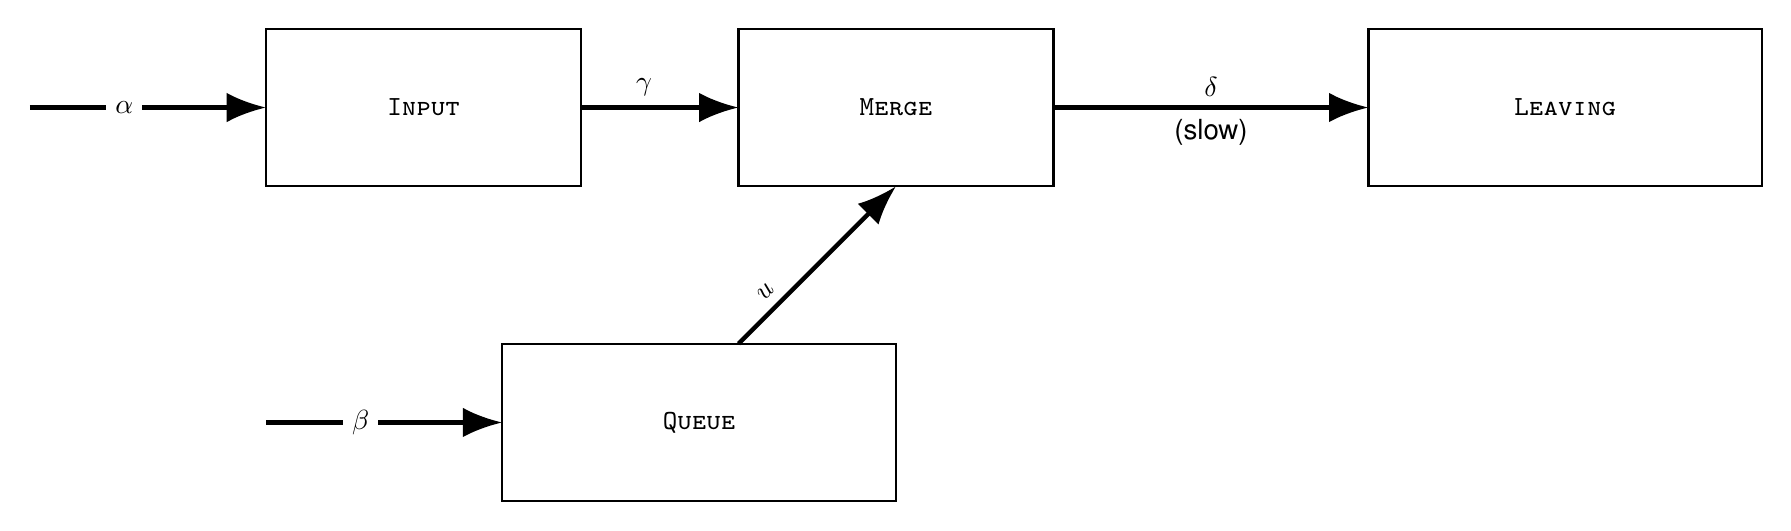
\begin{tikzpicture}
                    \draw[thick] (0,0) rectangle ++(4,2) node[midway] {\textsc{\texttt{Input}}};
                    \draw[thick] (6,0) rectangle ++(4,2) node[midway] {\textsc{\texttt{Merge}}};
                    \draw[thick] (14,0) rectangle ++(5,2) node[midway] {\textsc{\texttt{Leaving}}};
                    \draw[thick] (3,-4) rectangle ++(5,2) node[midway] {\textsc{\texttt{Queue}}};
                    \draw[-{Latex[length=5mm]}, ultra thick] (-3, 1) -- (0, 1) node[pos=.4, fill=white] {$\alpha$};
                    \draw[-{Latex[length=5mm]}, ultra thick] (0, -3) -- (3, -3) node[pos=.4, fill=white] {$\beta$};
                    \draw[-{Latex[length=5mm]}, ultra thick] (4, 1) -- (6, 1) node[pos=.4,above] {$\gamma$};
                    \draw[-{Latex[length=5mm]}, ultra thick] (10, 1) -- (14, 1) node[midway,above] {$\delta$} node[midway,below] {(slow)};
                    \draw[-{Latex[length=5mm]}, ultra thick] (6,-2) -- (8,0) node[near start,sloped,above] {$u$};
                \end{tikzpicture}
                \vspace{5mm}
            \end{center}
        
        \begin{center}
        \LARGE{\textbf{The approach}}
        \end{center}
            \large
        
            Describe what you are going to try and accomplish
	As the sun dipped below the horizon, casting hues of orange and pink across the sky, the quaint village came to life with the soft chatter of its inhabitants. Children chased each other through narrow cobblestone streets, their laughter echoing against the ancient stone walls. The scent of freshly baked bread wafted from the local bakery, enticing passersby with its warm embrace. In the distance, the sound of church bells rang out, signaling the end of another peaceful day in this idyllic countryside retreat.


            
            \FancyFigure{./imgs/img}{Figure caption.}{fig:evolution-comparison}
        
        \begin{center}
        \vspace{2cm}
        \LARGE{\textbf{Another heading}}
        \end{center}
            \large
        
            As the sun dipped below the horizon, casting hues of orange and pink across the sky, the quaint village came to life with the soft chatter of its inhabitants. Children chased each other through narrow cobblestone streets, their laughter echoing against the ancient stone walls. The scent of freshly baked bread wafted from the local bakery, enticing passersby with its warm embrace. In the distance, the sound of church bells rang out, signaling the end of another peaceful day in this idyllic countryside retreat.


        \columnbreak
        \begin{center}
        \LARGE{\textbf{Infinite-Time LQR}}
        \end{center}

            Only if you actually used Infinite-Time LQR?
As the sun dipped below the horizon, casting hues of orange and pink across the sky, the quaint village came to life with the soft chatter of its inhabitants. Children chased each other through narrow cobblestone streets, their laughter echoing against the ancient stone walls. The scent of freshly baked bread wafted from the local bakery, enticing passersby with its warm embrace. In the distance, the sound of church bells rang out, signaling the end of another peaceful day in this idyllic countryside retreat.


    \FancySubtitle[4mm][1cm]{Early Results \& Analysis}
    
        \begin{center}
          \includegraphics[width=1\linewidth,trim={0 8cm 0 10cm},clip]{./imgs/img.png}
        \end{center}
        
        As the sun dipped below the horizon, casting hues of orange and pink across the sky, the quaint village came to life with the soft chatter of its inhabitants. Children chased each other through narrow cobblestone streets, their laughter echoing against the ancient stone walls. The scent of freshly baked bread wafted from the local bakery, enticing passersby with its warm embrace. In the distance, the sound of church bells rang out, signaling the end of another peaceful day in this idyllic countryside retreat.

As the sun dipped below the horizon, casting hues of orange and pink across the sky, the quaint village came to life with the soft chatter of its inhabitants. Children chased each other through narrow cobblestone streets, their laughter echoing against the ancient stone walls. The scent of freshly baked bread wafted from the local bakery, enticing passersby with its warm embrace. In the distance, the sound of church bells rang out, signaling the end of another peaceful day in this idyllic countryside retreat.

          \columnbreak  
 As the sun dipped below the horizon, casting hues of orange and pink across the sky, the quaint village came to life with the soft chatter of its inhabitants. Children chased each other through narrow cobblestone streets, their laughter echoing against the ancient stone walls. The scent of freshly baked bread wafted from the local bakery, enticing passersby with its warm embrace. In the distance, the sound of church bells rang out, signaling the end of another peaceful day in this idyllic countryside retreat.

   \FancySubtitle[4mm][1cm]{Conclusions and next steps}
  As the sun dipped below the horizon, casting hues of orange and pink across the sky, the quaint village came to life with the soft chatter of its inhabitants. Children chased each other through narrow cobblestone streets, their laughter echoing against the ancient stone walls. The scent of freshly baked bread wafted from the local bakery, enticing passersby with its warm embrace. In the distance, the sound of church bells rang out, signaling the end of another peaceful day in this idyllic countryside retreat.
 As the sun dipped below the horizon, casting hues of orange and pink across the sky, the quaint village came to life with the soft chatter of its inhabitants. Children chased each other through narrow cobblestone streets, their laughter echoing against the ancient stone walls. The scent of freshly baked bread wafted from the local bakery, enticing passersby with its warm embrace. In the distance, the sound of church bells rang out, signaling the end of another peaceful day in this idyllic countryside retreat.

    \bibliographystyle{amsalpha}
    \bibliography{poster_references}
\end{multicols*}
\end{minipage}

\nocite{unsplash}
%Using nocite allows a reference to appear in the reference list without a citation appearing in the poster.
\footnotesize

\end{document}